\section{Ergebnisse} % (fold)
    \label{sec:ergebnisse}
    Text

    \begin{table}[h]
        \centering
        \caption{t-Test-Ergebnisse}
        \label{tab:t_test}
        \csvreader[tabular=rrr,
          table head=\toprule\centerIt{\textbf{Nullhypothese}} & \centerIt{\textbf{Sauer}} & \centerIt{\textbf{Salzig}}\\\midrule,
          /csv/separator=semicolon,
          head to column names,
          late after line=\\,
          late after last line=\\\bottomrule
          ]%
          {../Results/t_tests.csv}{H0=\H}%
        {\H & \pH & \NaCl}
    \end{table}
    Wie in \autoref{tab:t_test} zu sehen ist, \dots Die Quantile sind bla und bla\ \cite[vgl.][]{web:t-values} und bla\ \cite[vgl.][]{web:Gartenratgeber}\\

    \begin{figure}[ht]
        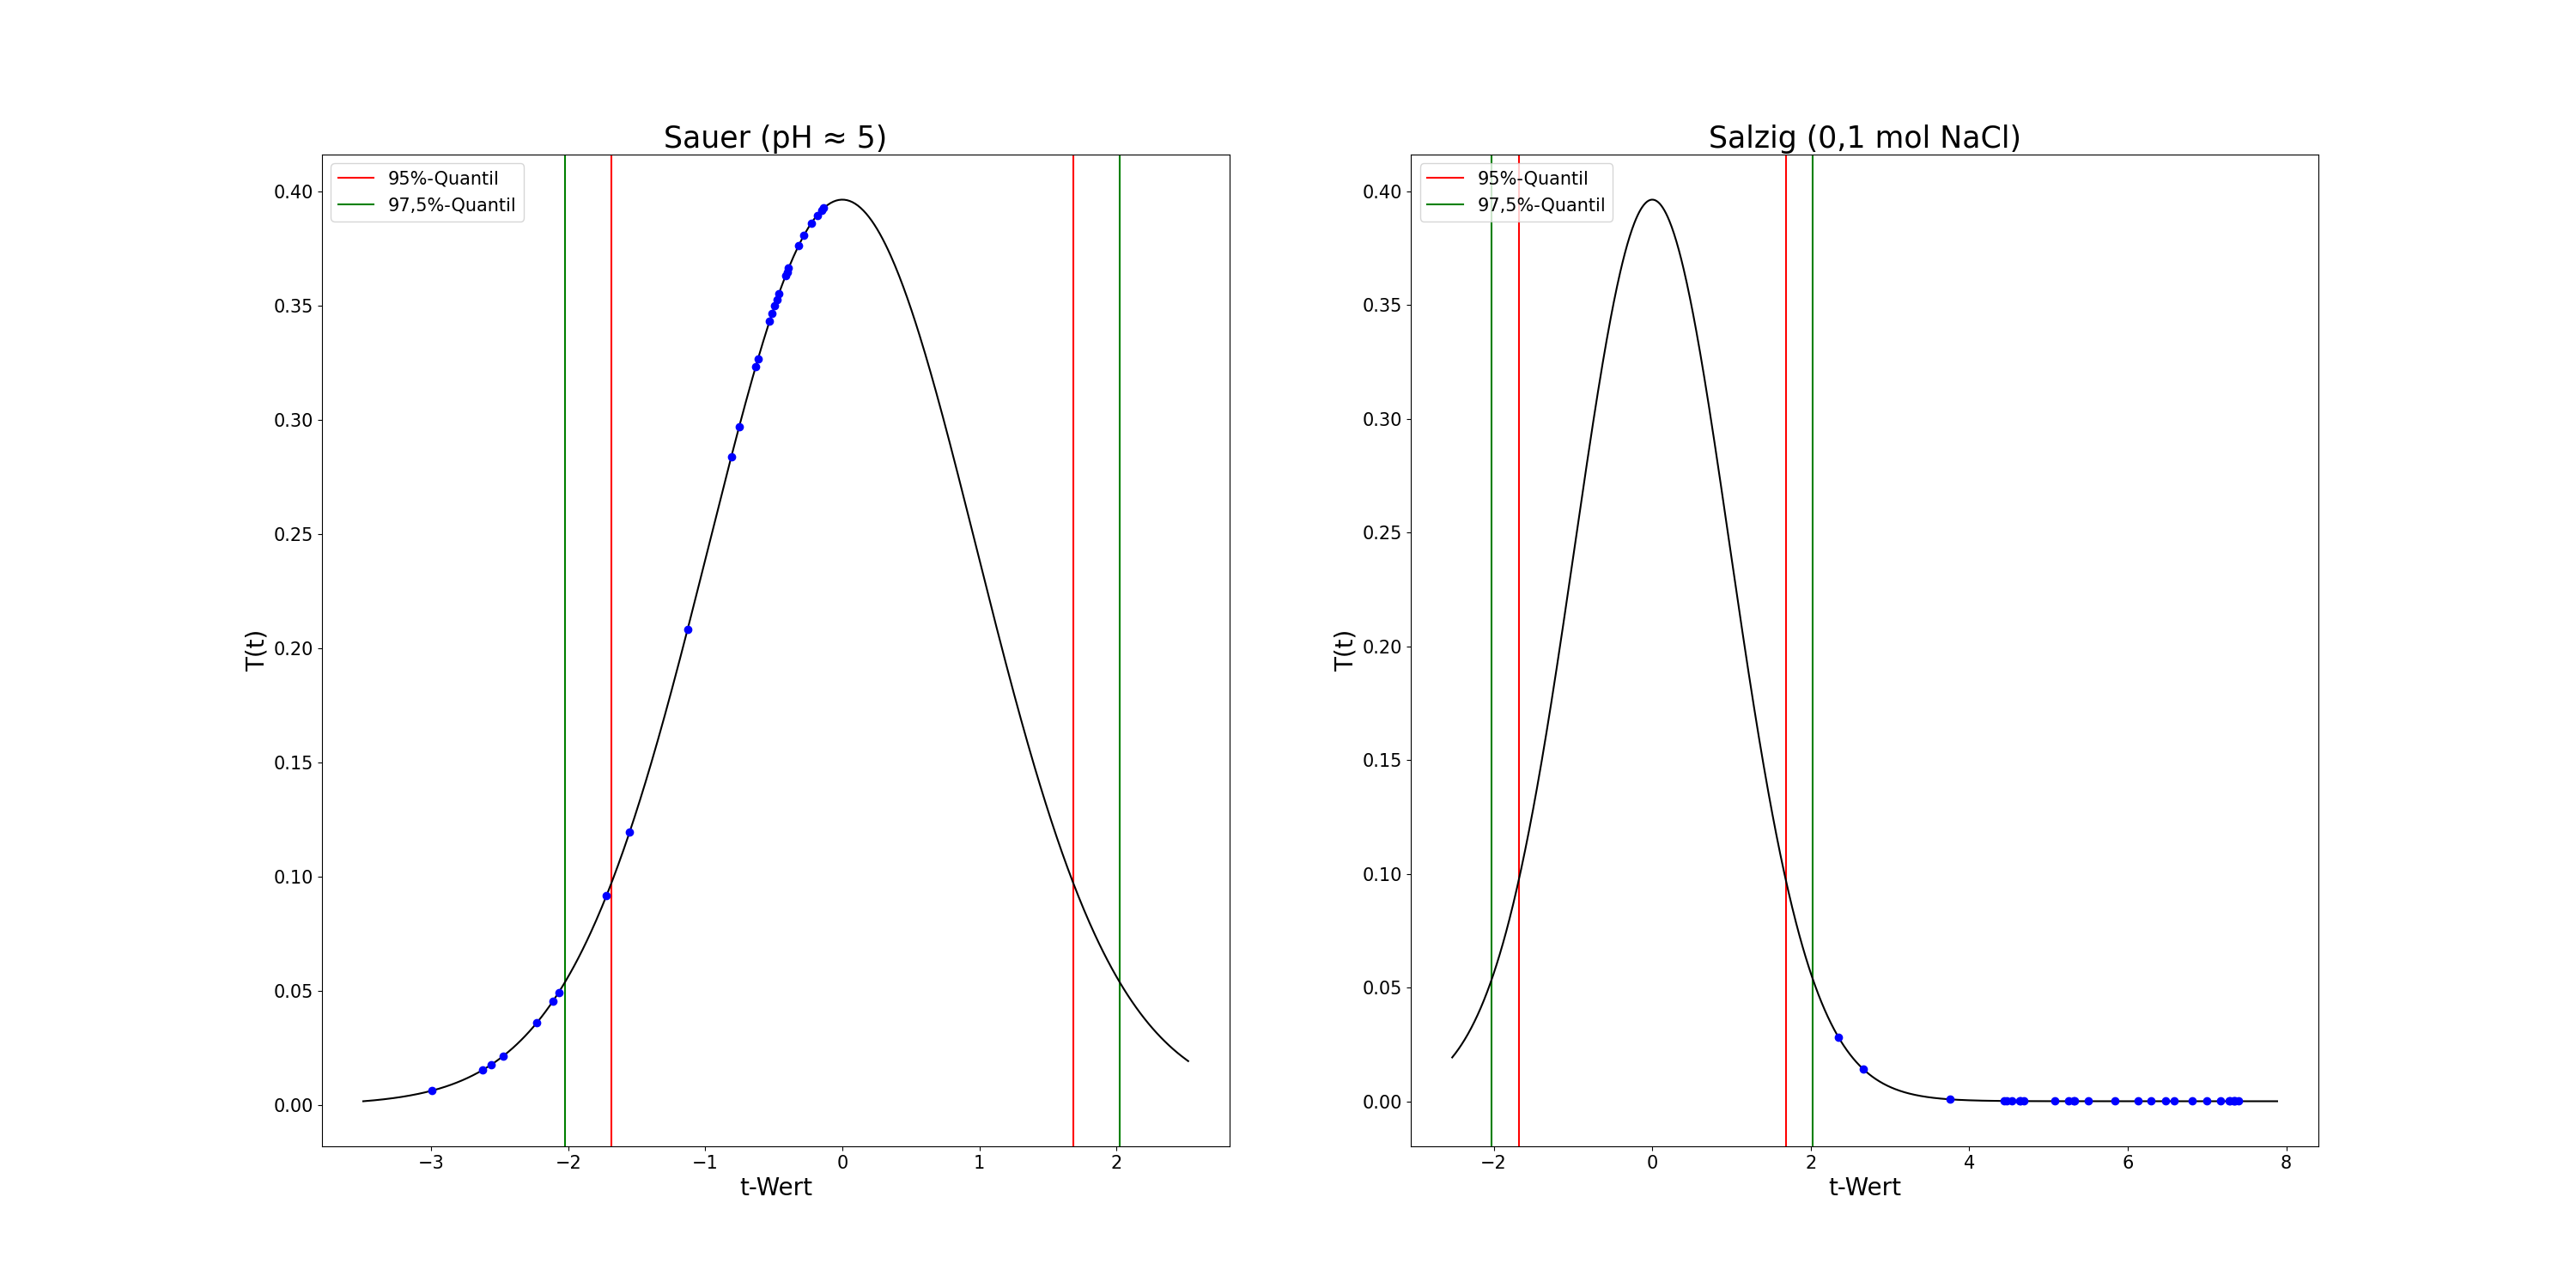
\includegraphics[width=1\textwidth]{t_tests.png}
        \caption{t-Tests}
        \label{fig:t_tests}
    \end{figure}
    asdasdasdasdasdasd\newpage

    \begin{figure}[ht]
        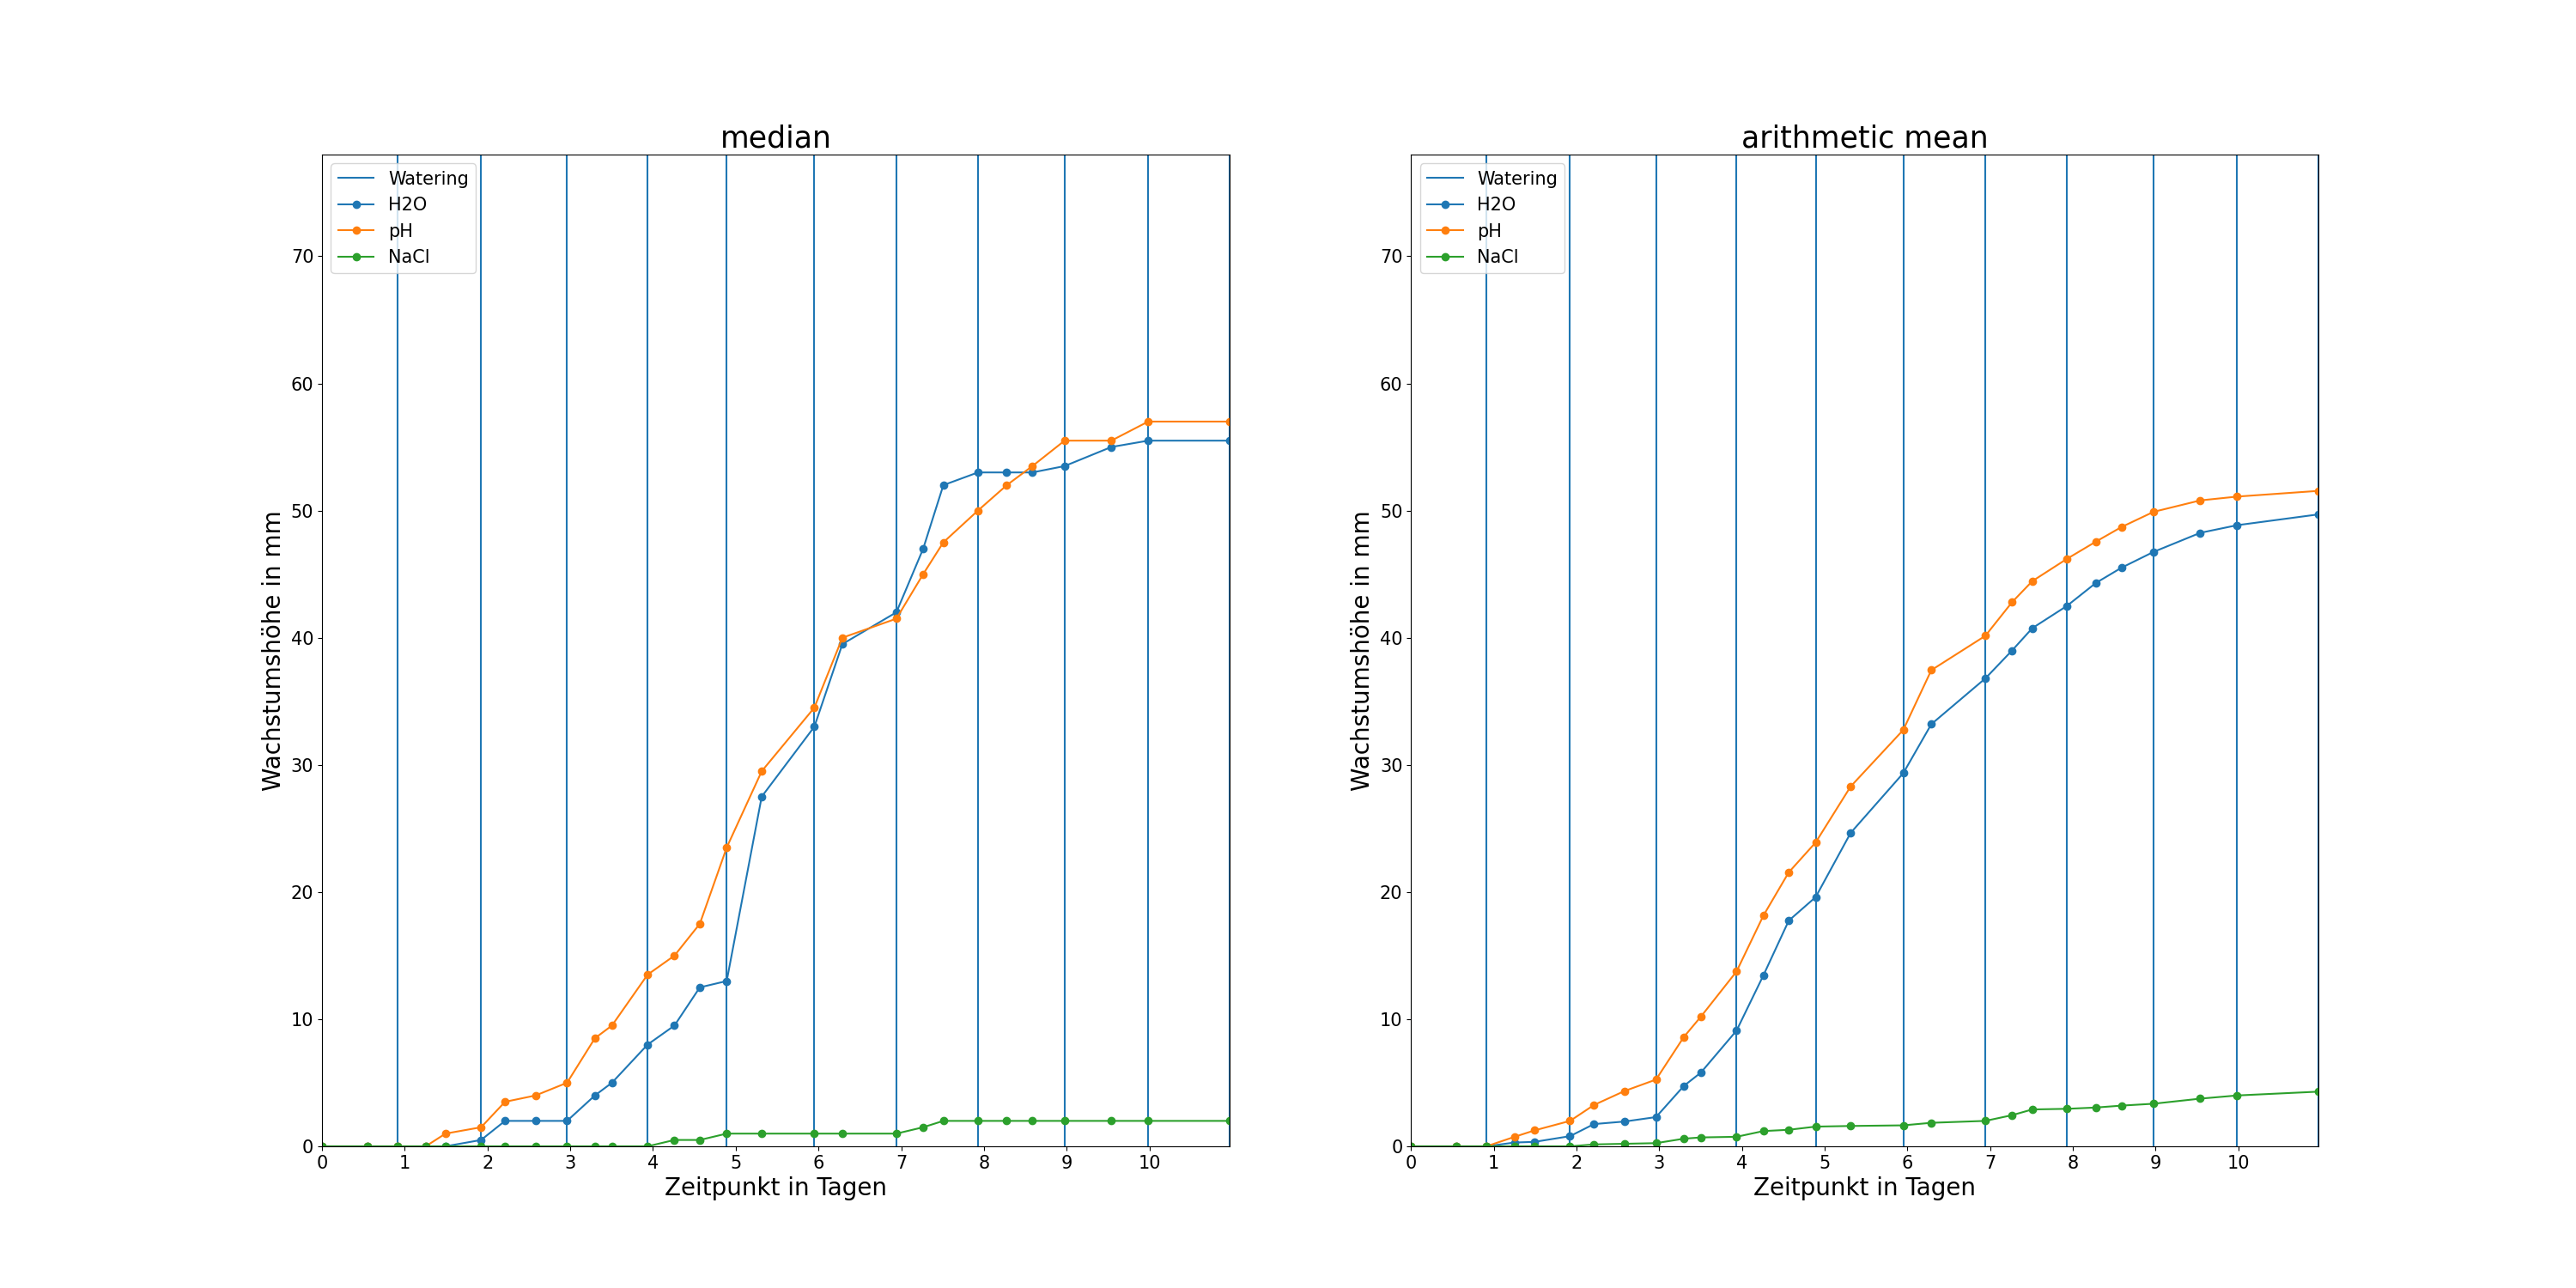
\includegraphics[width=1\textwidth]{ScatterPlot.png}
        \caption{Messwerte}
        \label{fig:scat_plot}
    \end{figure}\newpage

    \begin{figure}[ht]
        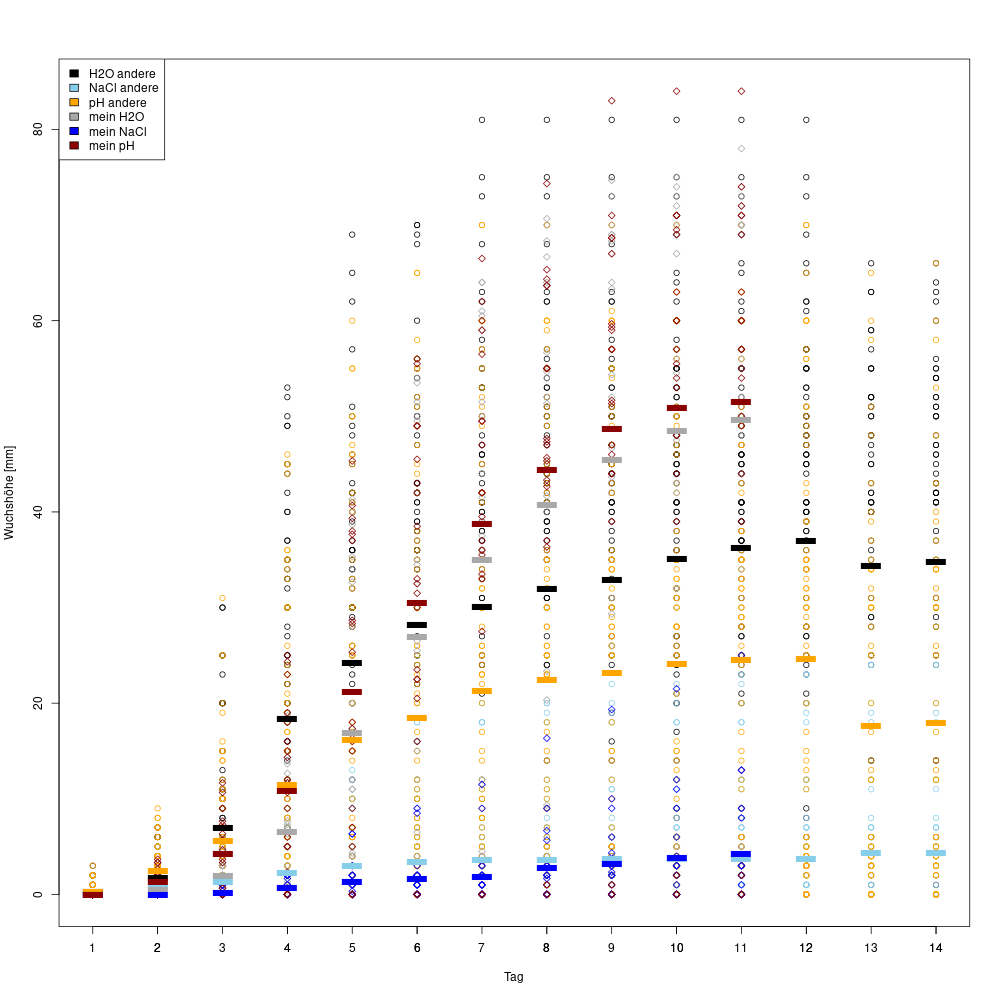
\includegraphics[width=1\textwidth]{scatterplot_my_vs_others.png}
        \caption{Wertevergleich mit anderen Durchführungen}
        \label{fig:scat_plot_cmp}
    \end{figure}
% section ergebnisse (end)
